\documentclass[11pt]{article}
\usepackage[margin=1in]{geometry}
\usepackage{amsmath,amssymb,bm}
\usepackage{graphicx}
\usepackage{booktabs}
\usepackage{hyperref}
\usepackage{tikz}
\newcommand{\e}{\mathbf{e}}
\newcommand{\rv}{\mathbf{r}}
\title{The Chaplygin Sleigh:\\ Lagrange--d'Alembert Equations, Reduction, and the Exact Solution}
\author{Michael Casey}
\date{October 25, 2026}
\begin{document}
\maketitle

\begin{abstract}
A planar rigid body rides on a knife-edge blade offset from its center of mass. The blade cannot slip sideways: a constraint linear in velocity that fails the Frobenius integrability condition, so the system is nonholonomic and the usual Lagrange equations do not apply. This note derives the equations of motion by the Lagrange--d'Alembert principle with a multiplier, reduces them to two first-order equations in the blade's forward speed and the yaw rate, solves those in closed form (speed, yaw rate and the total heading change), and shows that among the straight motions, which form a line of equilibria, those with the center of mass leading the blade are stable to yaw and attract their neighbours while those with it trailing are unstable. The MATLAB script \texttt{run\_sleigh.m} checks every step numerically.
\end{abstract}

\section{Setup and conventions}
World frame: $x$ east, $y$ north, heading $\theta$ counterclockwise from $x$. Body axes
\[
\e_1 = (\cos\theta,\ \sin\theta),\qquad \e_2 = (-\sin\theta,\ \cos\theta),\qquad \dot\e_1 = \omega\,\e_2,\quad \dot\e_2 = -\omega\,\e_1,\quad \omega = \dot\theta .
\]
The body has mass $m$ and inertia $J$ about its center of mass $\rv_c = (x_c, y_c)$. The blade touches the plane at
\[
\rv_b = \rv_c - a\,\e_1 ,
\]
so $a > 0$ puts the center of mass \emph{ahead} of the blade in the forward direction (Figure~\ref{fig:body}). The blade is a knife edge aligned with $\e_1$: it may slide along $\e_1$ and turn, but it cannot move along $\e_2$.

\begin{figure}[h]
\centering
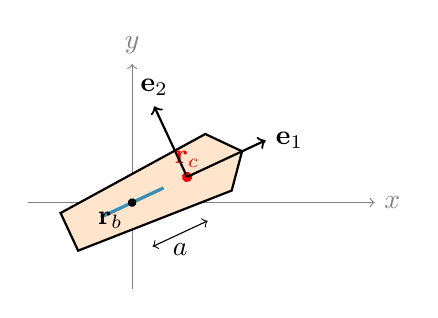
\begin{tikzpicture}[scale=2.2]
  \draw[->, gray] (-0.6,0) -- (1.4,0) node[right] {$x$};
  \draw[->, gray] (0,-0.5) -- (0,0.8) node[above] {$y$};
  \begin{scope}[rotate=25]
    \draw[thick, fill=orange!20] (0.7,0) -- (0.55,0.18) -- (-0.4,0.12) -- (-0.4,-0.12) -- (0.55,-0.18) -- cycle;
    \draw[very thick, cyan!70!black] (-0.2,0) -- (0.2,0);
    \fill (0,0) circle (0.025) node[below left] {$\rv_b$};
    \fill[red] (0.35,0) circle (0.03) node[above] {$\rv_c$};
    \draw[->, thick] (0.35,0) -- (0.85,0) node[right] {$\e_1$};
    \draw[->, thick] (0.35,0) -- (0.35,0.45) node[above] {$\e_2$};
    \draw[<->] (0,-0.28) -- (0.35,-0.28) node[midway, below] {$a$};
  \end{scope}
\end{tikzpicture}
\caption{The sleigh. The blade (cyan) sits at $\rv_b$ and is aligned with $\e_1$; the center of mass (red) is $a\,\e_1$ ahead of it.}
\label{fig:body}
\end{figure}

\section{Lagrange--d'Alembert with the multiplier}
Generalized coordinates $q = (x_c, y_c, \theta)$. There is no potential, so
\[
L = \tfrac{m}{2}\left(\dot x_c^2 + \dot y_c^2\right) + \tfrac{J}{2}\dot\theta^2,\qquad M = \mathrm{diag}(m, m, J).
\]
The blade's velocity is $\dot\rv_b = \dot\rv_c - a\omega\,\e_2$, and the knife edge demands $\dot\rv_b\cdot\e_2 = 0$:
\begin{equation}
A(q)\,\dot q = 0,\qquad A = \begin{bmatrix} -\sin\theta & \cos\theta & -a \end{bmatrix}.
\label{eq:constraint}
\end{equation}
Is this constraint holonomic in disguise? A one-form $\alpha$ defines a holonomic constraint when some integrating factor makes it exact, and Frobenius' theorem says that happens if and only if $\alpha\wedge d\alpha = 0$. Here $\alpha = -\sin\theta\,dx_c + \cos\theta\,dy_c - a\,d\theta$, $d\alpha = -\cos\theta\,d\theta\wedge dx_c - \sin\theta\,d\theta\wedge dy_c$, and
\[
\alpha\wedge d\alpha = -\,dx_c\wedge dy_c\wedge d\theta \neq 0
\]
for every $a$, including $a = 0$. So no coordinate change turns \eqref{eq:constraint} into a condition on positions: the sleigh has three configuration degrees of freedom but only two velocity degrees of freedom. (Non-closedness alone would not prove this: $e^x\,dy$ is not closed, yet its zero set is $\dot y = 0$.) The Lagrange--d'Alembert principle states that the constraint force does no work on admissible velocities, which puts it in the row space of $A$:
\begin{equation}
\frac{d}{dt}\frac{\partial L}{\partial \dot q} - \frac{\partial L}{\partial q} = A^{\!\top}\lambda
\quad\Longrightarrow\quad
m\ddot x_c = -\lambda\sin\theta,\qquad m\ddot y_c = \lambda\cos\theta,\qquad J\ddot\theta = -a\lambda .
\label{eq:LdA}
\end{equation}
$\lambda$ is the sideways force the ice exerts on the blade, along $\e_2$, and $-a\lambda$ is its moment about the center of mass. In general, with $p = \partial L/\partial\dot q$, $M = \partial p/\partial\dot q$ and $h = (\partial p/\partial q)\,\dot q - \partial L/\partial q$ (the Euler--Lagrange terms left after removing $M\ddot q$, for an autonomous $L$), and with generalized forces $Q$, the equations are $M\ddot q + h = Q + A^{\!\top}\lambda$. Together with the time derivative of the constraint, $A\ddot q + \dot A\dot q = 0$, the unknowns $(\ddot q, \lambda)$ satisfy the block system
\[
\begin{bmatrix} M & A^{\!\top} \\ A & 0 \end{bmatrix}
\begin{bmatrix} \ddot q \\ -\lambda \end{bmatrix} =
\begin{bmatrix} Q - h \\ -\dot A\dot q \end{bmatrix},
\]
which is what \texttt{mech.lagrange\_dalembert} solves symbolically for any $L$, $A$ and $Q$ with $M$ nonsingular and $A$ of full row rank. For the sleigh $Q = 0$ and $h = 0$ (Cartesian coordinates, no potential), and the top block reduces to \eqref{eq:LdA}.

\section{Reduction to the blade's speed and the yaw rate}
Define the quasi-velocities $v = \dot\rv_b\cdot\e_1 = \dot x_c\cos\theta + \dot y_c\sin\theta$ (the forward speed, the same for blade and center of mass) and $\omega = \dot\theta$. The constraint gives $\dot\rv_c = v\,\e_1 + a\omega\,\e_2$, and differentiating,
\[
\ddot\rv_c = (\dot v - a\omega^2)\,\e_1 + (v\omega + a\dot\omega)\,\e_2 .
\]
Comparing with $m\ddot\rv_c = \lambda\,\e_2$ from \eqref{eq:LdA}: the $\e_1$ component gives $\dot v = a\omega^2$ and the $\e_2$ component $\lambda = m(v\omega + a\dot\omega)$. Substituting into $J\dot\omega = -a\lambda$ and collecting $\dot\omega$,
\begin{equation}
\boxed{\;\dot v = a\,\omega^2,\qquad \dot\omega = -k\,v\,\omega,\qquad k = \frac{m a}{J + m a^2},\qquad \lambda = \frac{m J}{J + m a^2}\,v\,\omega\;}
\label{eq:reduced}
\end{equation}
with the kinematics $\dot x_b = v\cos\theta$, $\dot y_b = v\sin\theta$, $\dot\theta = \omega$. The script integrates this five-state system (\texttt{sleigh\_rhs}). The symbolic builder, given only $L$ and $A$, returns for the defaults $m = 1$, $J = 0.1$, $a = 0.2$ (so $mJ/(J + ma^2) = 5/7$)
\begin{align*}
\ddot q &= \frac{5\,\dot\theta\,(\dot x_c\cos\theta + \dot y_c\sin\theta)}{7}
\begin{bmatrix} -\sin\theta \\ \phantom{-}\cos\theta \\ -2 \end{bmatrix},\\
\lambda &= \frac{5\,\dot\theta\,(\dot x_c\cos\theta + \dot y_c\sin\theta)}{7},
\end{align*}
(the builder prints the three components of $\ddot q$ separately, each with the factor $5\dot\theta(\dot x_c\cos\theta + \dot y_c\sin\theta)/7$ and the entries $-\sin\theta$, $\cos\theta$, $-2$; they are grouped here). Since $v = \dot x_c\cos\theta + \dot y_c\sin\theta$, the string is $\lambda = \tfrac{5}{7}v\omega$, matching \eqref{eq:reduced}, and the script compares the two pointwise along the solution (line D1).

\section{Energy, the invariant ellipse, and the exact solution}
The kinetic energy about the center of mass, with $|\dot\rv_c|^2 = v^2 + a^2\omega^2$, is
\begin{equation}
E = \tfrac{m}{2}v^2 + \tfrac{1}{2}(J + m a^2)\,\omega^2 ,
\label{eq:energy}
\end{equation}
and \eqref{eq:reduced} conserves it: $\dot E = m v\,a\omega^2 - (J + ma^2)\,k\,v\,\omega^2 = 0$ since $(J + ma^2)k = ma$. So the motion in the $(v, \omega)$ plane stays on the ellipse
\[
v^2 + \frac{J + m a^2}{m}\,\omega^2 = C,\qquad C = v_0^2 + \frac{J + m a^2}{m}\,\omega_0^2 .
\]
Eliminating $\omega^2$ from $\dot v = a\omega^2$ gives $\dot v = k\,(C - v^2)$, a Riccati equation. For $a \neq 0$ and $\omega_0 \neq 0$, write $b = \sqrt{(J + ma^2)/m}$, $S = \sqrt{C}$ and
\begin{equation}
z(t) = \alpha + kS\,t,\qquad \alpha = \operatorname{arsinh}\!\frac{v_0}{b\,|\omega_0|},\qquad
v(t) = S\tanh z,\qquad \omega(t) = \operatorname{sign}(\omega_0)\,\frac{S}{b}\,\operatorname{sech} z .
\label{eq:exact}
\end{equation}
At $t = 0$ this returns $v_0$ and $\omega_0$ (since $\tanh\alpha = v_0/S$ and $\cosh\alpha = S/(b|\omega_0|)$), and it is the form to evaluate numerically: the equivalent $v = S\tanh(kS(t - t_0))$ with $t_0 = -\operatorname{artanh}(v_0/S)/(kS)$ fails for tiny $\omega_0$, where $C$ rounds to $v_0^2$ and $\operatorname{artanh}(\pm 1)$ is infinite. $\omega$ never changes sign (its equation is linear in $\omega$; equivalently $\omega = \omega_0\exp(-k\int_0^t v)$), and $v \to \operatorname{sign}(a)\,S$. The heading also integrates exactly, since $\int\operatorname{sech} z\,dz$ is the Gudermannian:
\begin{equation}
\theta_\infty - \theta_0 = \operatorname{sign}(\omega_0)\,\frac{b}{|a|}\,\arccos\!\frac{\operatorname{sign}(a)\,v_0}{S},
\label{eq:heading}
\end{equation}
which can exceed several revolutions when $|a|$ is small. Two special cases fall outside \eqref{eq:exact}: $a = 0$ is the knife edge, $k = 0$, $v$ and $\omega$ constant and the blade runs a circle of radius $|v_0/\omega_0|$ with $\lambda = m v\omega$ the centripetal force; $\omega_0 = 0$ is the straight ride at constant $v_0$ for every $a$, whether or not it is stable. Line D2 of the script measures the integrator against \eqref{eq:exact}, D3 against \eqref{eq:energy}, D5 against \eqref{eq:heading}; D4 evaluates \eqref{eq:constraint} on the reconstructed center-of-mass velocity $\dot\rv_c = v\e_1 + a\omega\e_2$, where it vanishes identically, so D4 is a consistency check of that mapping rather than independent evidence.

\section{Stability of straight motion}
Straight motion ($\omega = 0$, $v = V$) is a whole line of equilibria of \eqref{eq:reduced}, one for each speed. Linearizing at $(V, 0)$,
\[
\begin{bmatrix}\delta\dot v\\ \delta\dot\omega\end{bmatrix} = \begin{bmatrix} 0 & 0\\ 0 & -kV\end{bmatrix}\begin{bmatrix}\delta v\\ \delta\omega\end{bmatrix},
\]
and the zero eigenvalue is real: a perturbation $\delta v$ along the line is itself another equilibrium and never decays, so no single straight motion is asymptotically stable in the $(v, \omega)$ plane. The transverse eigenvalue $-kV$ is what the sign of $a$ decides. When $aV > 0$, the center of mass ahead of the blade in the direction of travel, a yaw perturbation decays and the motion converges to a nearby straight ride at the speed its energy allows: the equilibrium is Lyapunov stable and transversely attracting, and on its own energy ellipse it is asymptotically stable. When $aV < 0$ it is unstable to yaw. The exact solution says the same globally: for $a \neq 0$ and any $\omega_0 \neq 0$, however small, the sleigh ends up moving at $\operatorname{sign}(a)\,S$. A sleigh launched with the center of mass trailing therefore sees $|\omega|$ \emph{grow} (to $S/b$ at the moment $v = 0$), its signed speed cross zero exactly once, at $t_{\rm rev} = -\operatorname{artanh}(v_0/S)/(kS)$, and then departs along the stable direction, turning in total by \eqref{eq:heading} (Figure~\ref{fig:paths}). With $\omega_0 = 0$ exactly, nothing happens: the trailing straight ride is an exact, unstable equilibrium.

No energy is dissipated in this model. The constraint force does no work in total, $\lambda\e_2\cdot\dot\rv_c + (-a\lambda)\omega = a\lambda\omega - a\lambda\omega = 0$, and the kinetic energy \eqref{eq:energy} is conserved. What changes is its split: the rotational part $\tfrac{J}{2}\omega^2$ obeys $\tfrac{d}{dt}\tfrac{J}{2}\omega^2 = -Jk\,v\,\omega^2$, so it decreases when $av > 0$ and increases when $av < 0$, the translational part changing by the opposite amount. Yaw is traded into forward motion through the constraint, reversibly, not dissipated. The energy-split panel of Figure~\ref{fig:diag} shows exactly this trade.

\begin{figure}[h]
\centering
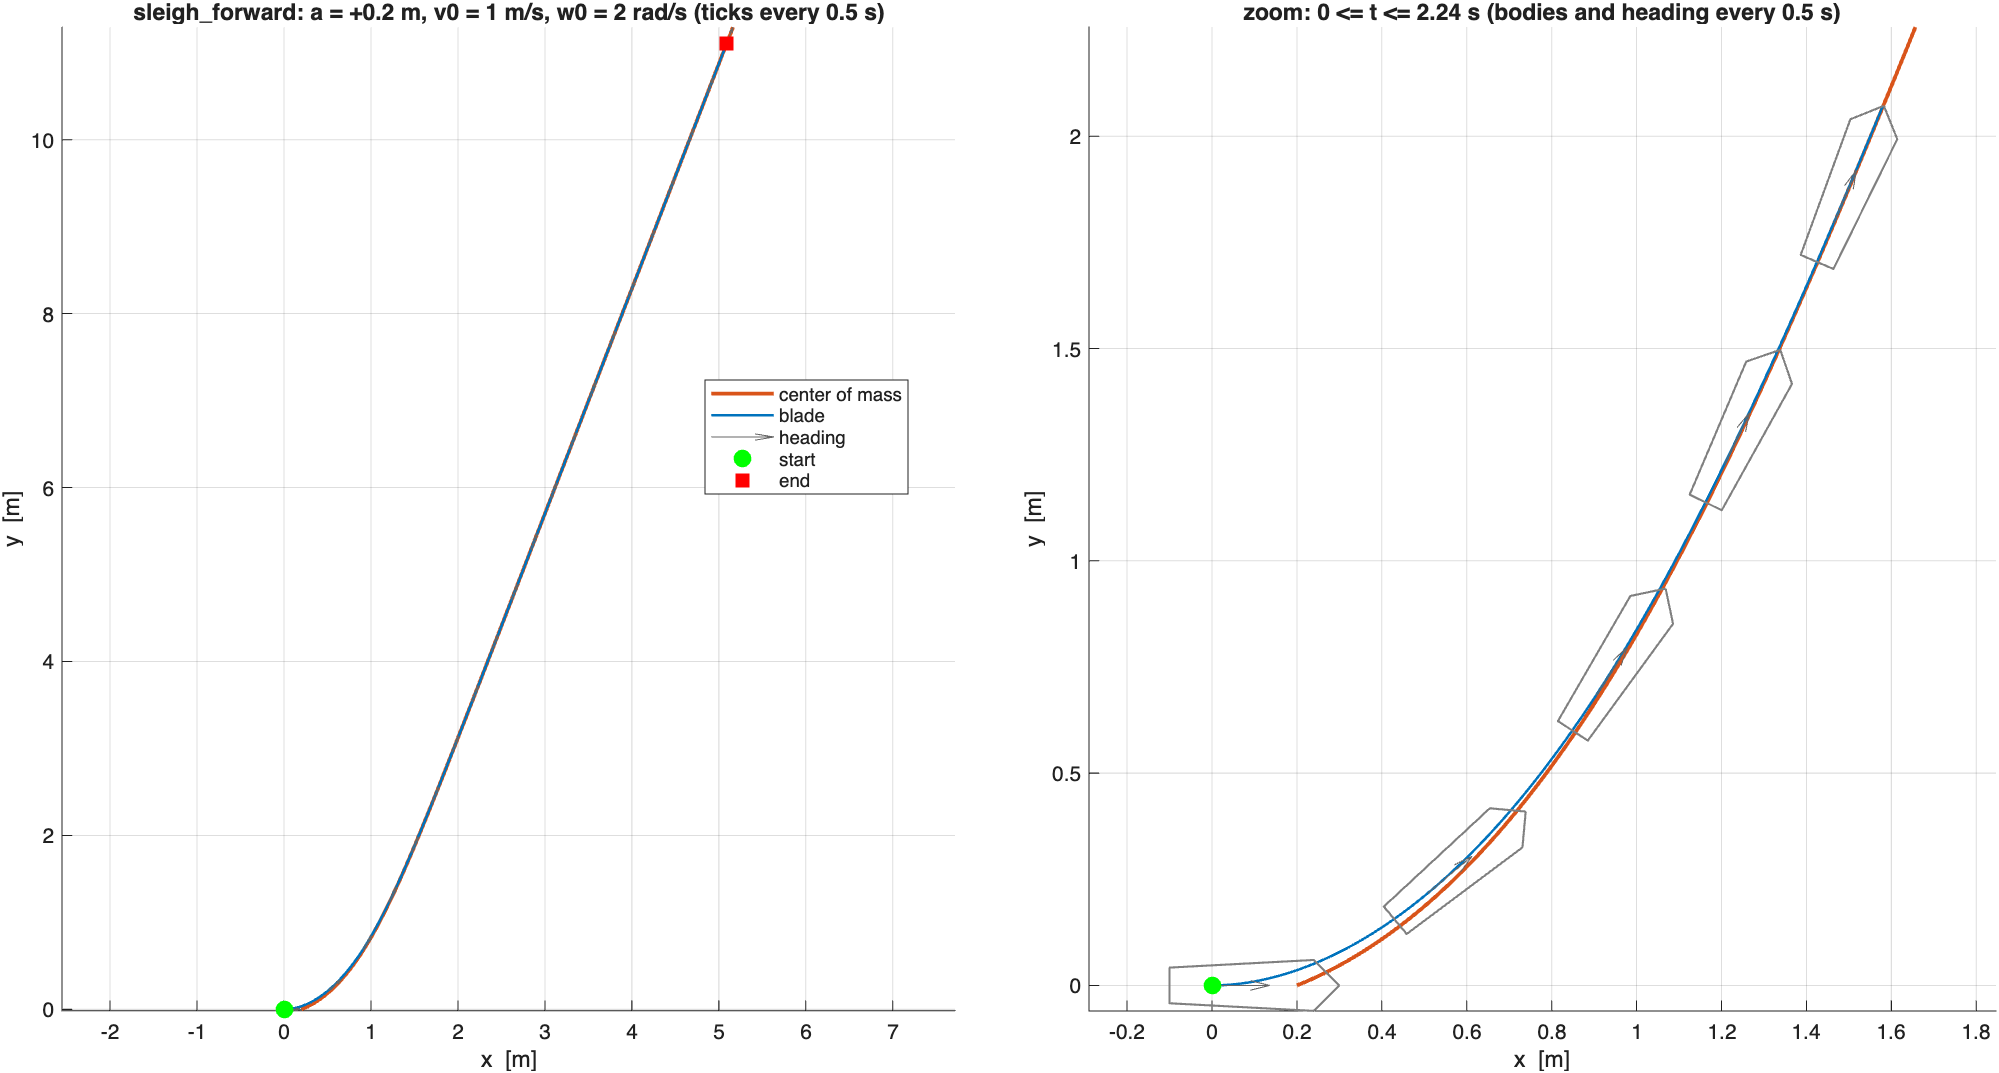
\includegraphics[width=\textwidth]{figures/sleigh_forward_path.png}\\[4pt]
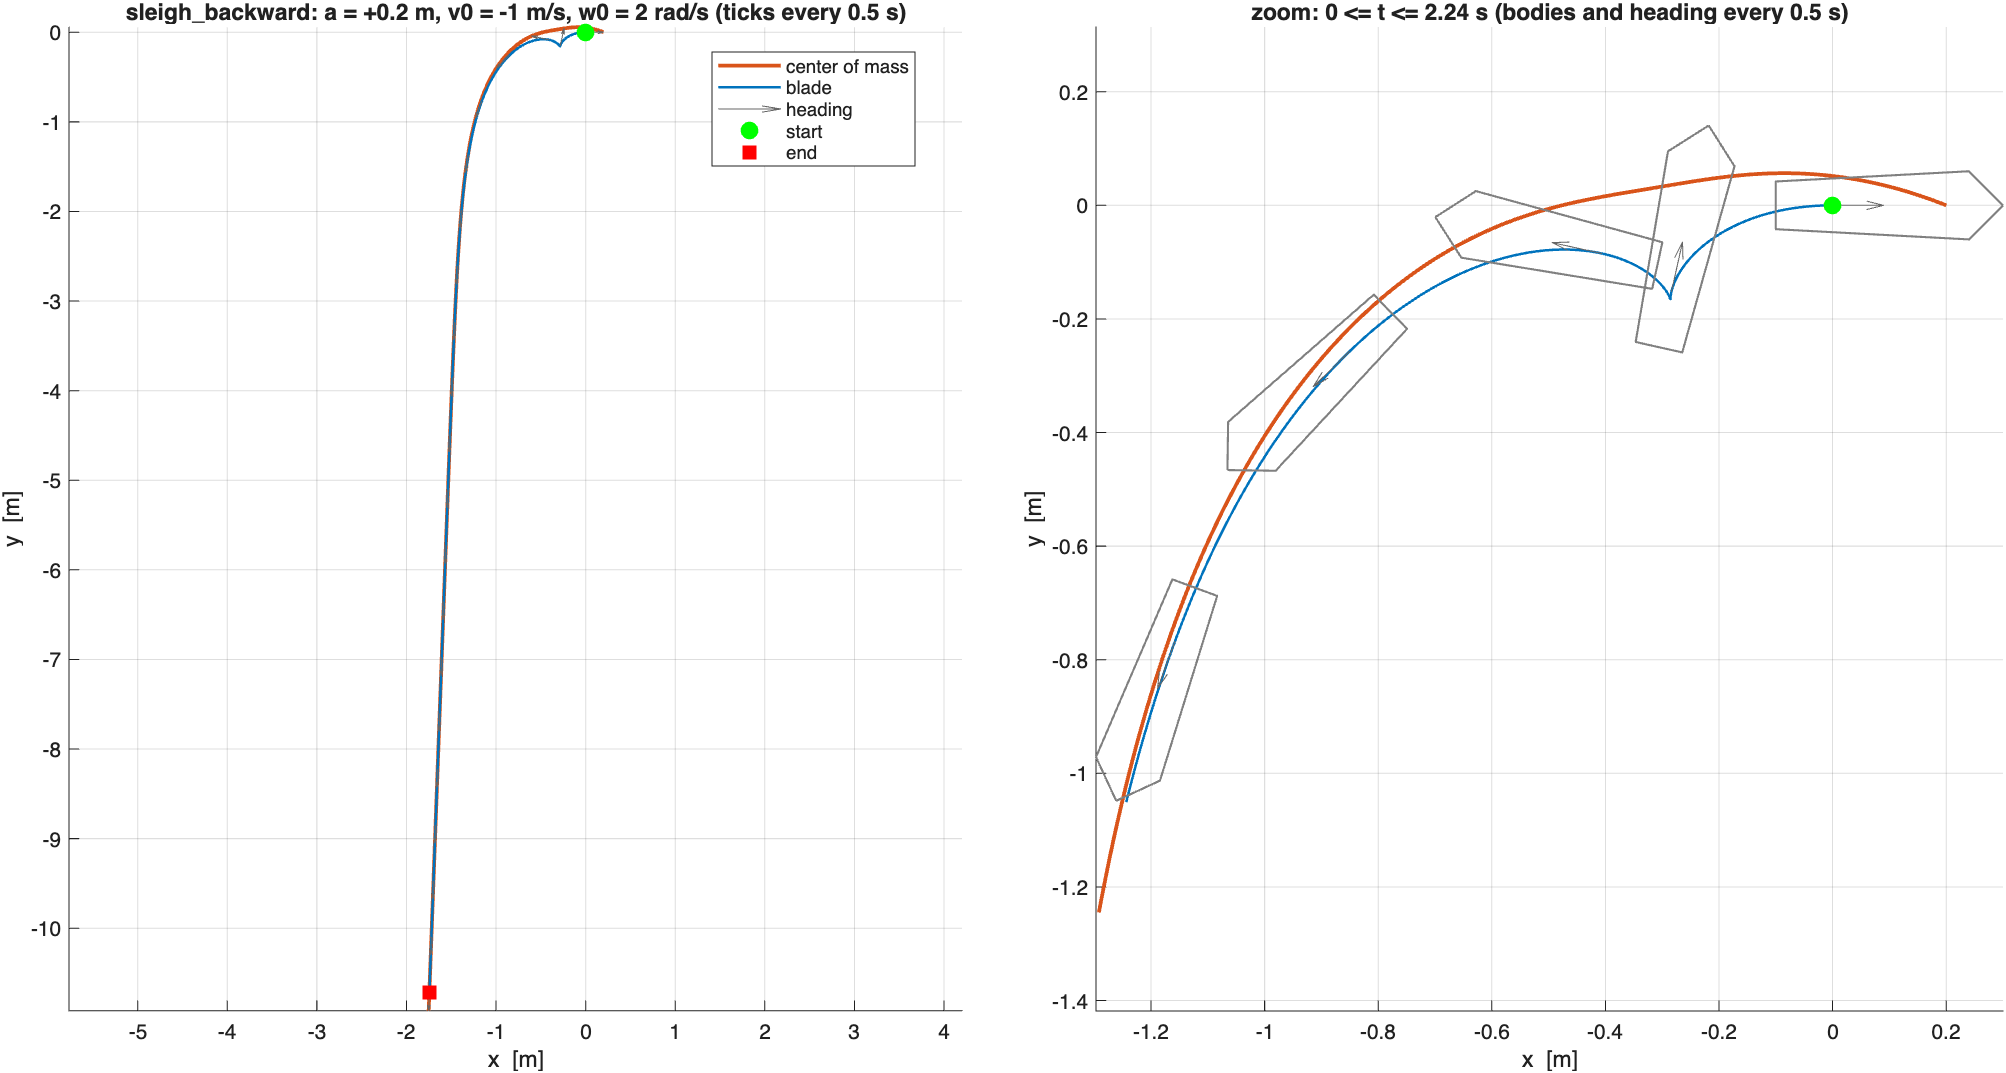
\includegraphics[width=\textwidth]{figures/sleigh_backward_path.png}
\caption{Paths of the center of mass and the blade for $a = 0.2$~m and $\omega_0 = 2$~rad/s; each image shows the whole path (left pane) and a zoom over the first few time constants with the body drawn at every 0.5~s tick (right pane). (top) $v_0 = +1$~m/s: the center of mass leads, the heading turns by $1.20$~rad in total and the ride straightens. (bottom) $v_0 = -1$~m/s: it trails, $|\omega|$ grows, the signed speed crosses zero at $0.617$~s, and the sleigh departs the other way after turning $4.68$~rad in total.}
\label{fig:paths}
\end{figure}

\section{Numerical check}
Figure~\ref{fig:diag} is the diagnostics panel of \texttt{run\_sleigh.m} for the defaults. The printed verdicts of that run were:
\begin{verbatim}
PASS  D1 hand-derived vs builder: 8.88e-16 (bar 1e-09)
PASS  D2 exact solution (v, w): 4.71e-13 (bar 1e-08)
PASS  D3 energy drift (rel): 7.81e-14 (bar 1e-09)
PASS  D4 constraint residual |A qd|: 2.22e-16 (bar 1e-09)
PASS  D5 asymptotics: v -> sign(a) sqrt(C) = +1.249000 (v(end) +1.249000),
      |w(end)| = 4.0e-08, heading change 1.2019 rad vs exact 1.2019
\end{verbatim}
(Line D5 continues in the script output with the stability verdict for the center of mass leading; it is wrapped here for the page.)

\begin{figure}[h]
\centering
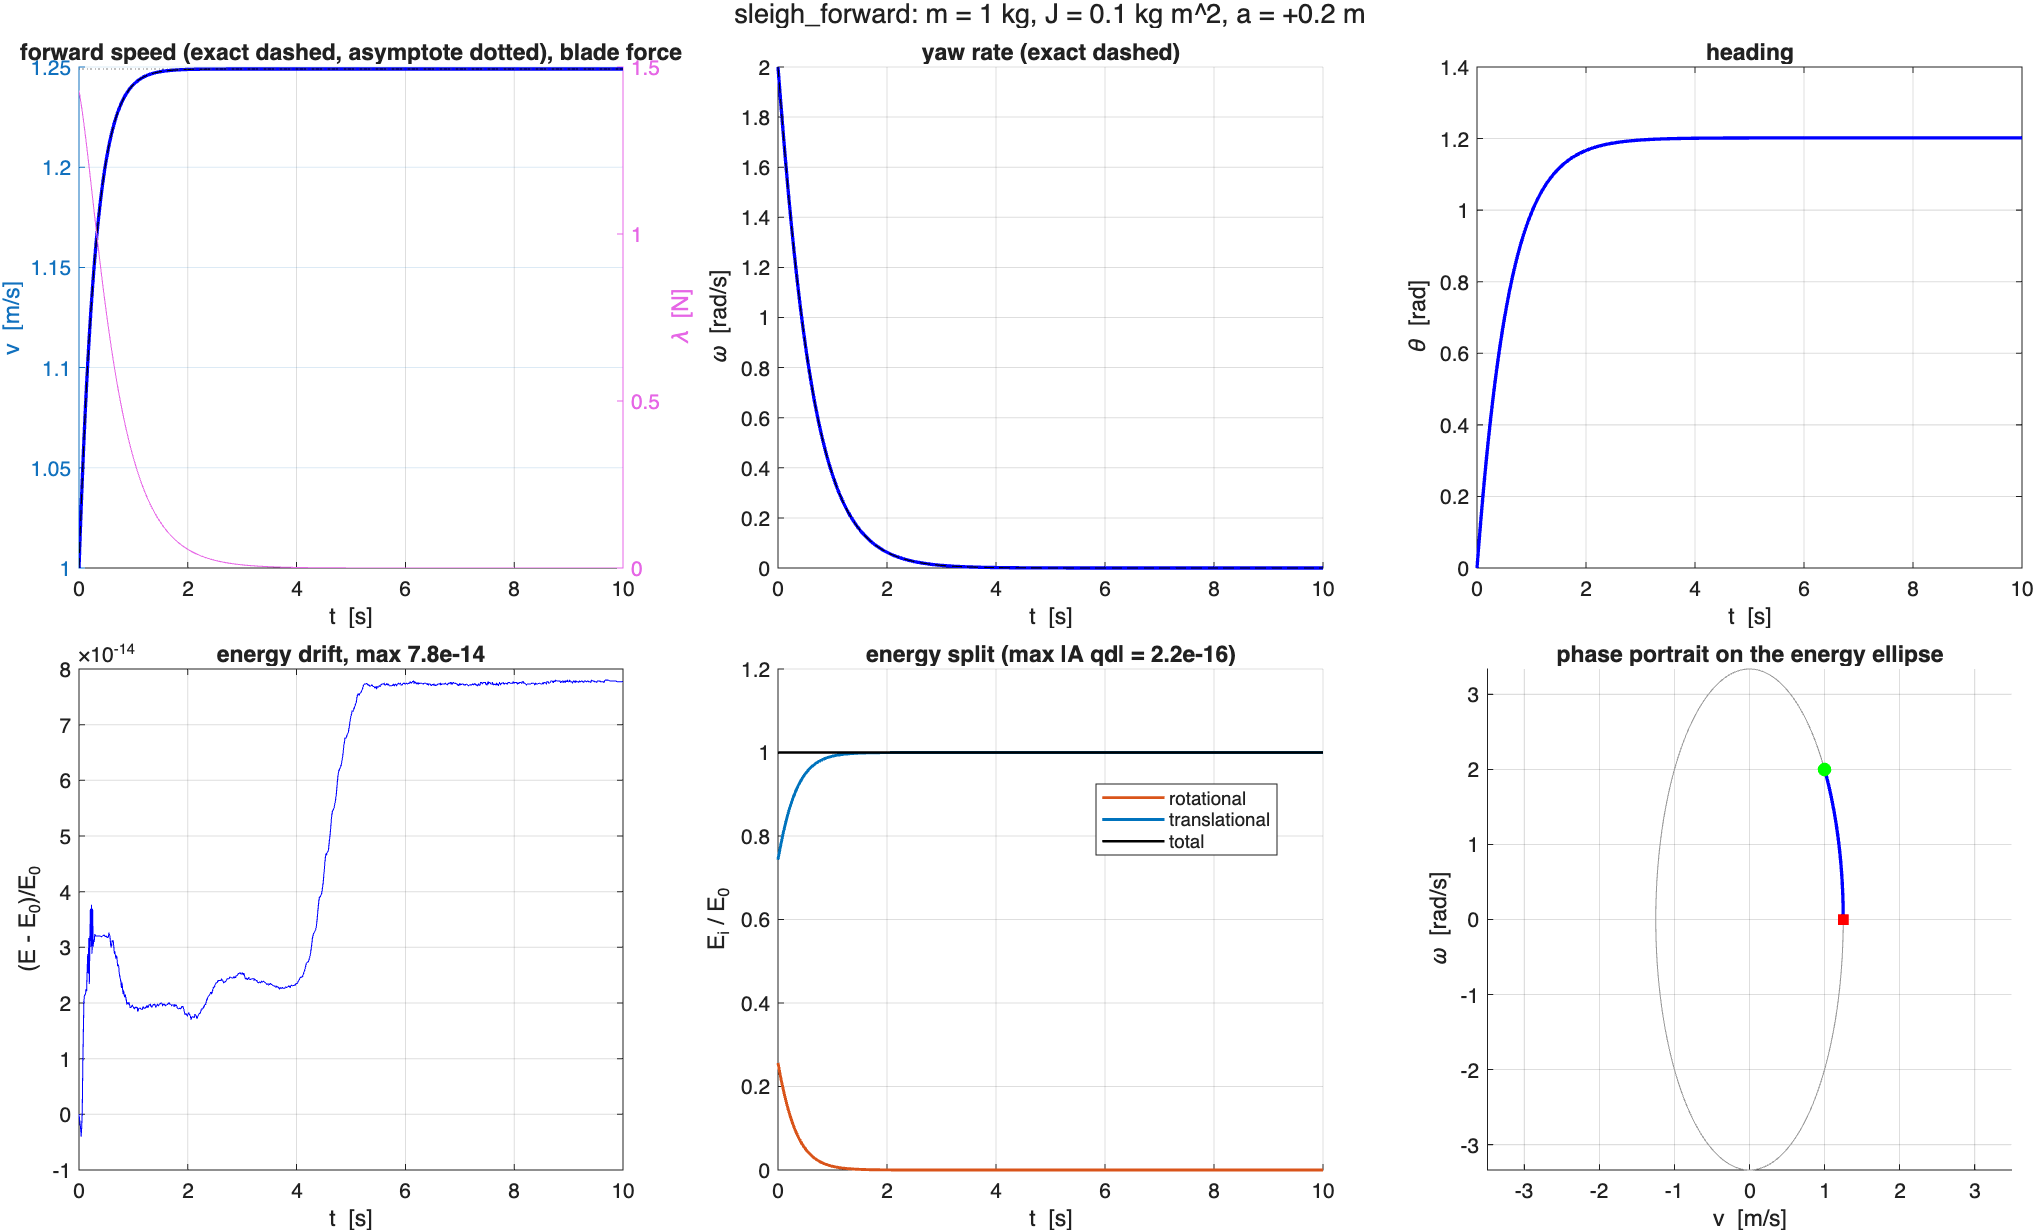
\includegraphics[width=\textwidth]{figures/sleigh_forward_diag.png}
\caption{Forward speed with the exact solution and the asymptote, yaw rate, heading, energy drift, the energy split (rotational, translational, total; the yaw energy is traded into translation, the total is flat), and the $(v,\omega)$ phase portrait on its energy ellipse.}
\label{fig:diag}
\end{figure}

\section*{References}
\small
\begin{enumerate}
\item A. M. Bloch, \emph{Nonholonomic Mechanics and Control}, 2nd ed., Springer, 2015, Sections 1.4 and 1.7.
\item Ju. I. Neimark and N. A. Fufaev, \emph{Dynamics of Nonholonomic Systems}, AMS Translations of Mathematical Monographs 33, 1972.
\item S. A. Chaplygin, ``On the theory of motion of nonholonomic systems. The reducing-multiplier theorem,'' \emph{Mat. Sbornik} 28, 1911 (English translation in \emph{Regular and Chaotic Dynamics} 13, 2008).
\end{enumerate}
\end{document}
